\section{Competition creates research}\label{sec:09_research}

So far the investor is present with a fixed probability \(\lambda\). Section~5 of the paper lets the investor choose
that probability and pay for it. Over a range of strengths, research, entry and high-class ownership then rise together
with the incumbent's strength. The prior is \(1/2\) throughout.
Use rule C1 unless the text states rule CM.

\subsection{Research as chosen presence}\label{sec:09_research-setup}

Before it learns the class, the investor chooses a research intensity \(\lambda\in[0,\lb]\) at the cost
\((a/2)\lambda^2\), with \(a>0\) and a cap \(0<\lb<1\). Research succeeds with probability \(\lambda\), independently of
the class, the costs and the incumbent's value. A success reveals the class, and the investor fills the slot with an
order. After a failure a liquidity trader fills the slot. So research is the presence probability of the order slot,
chosen at a cost. The cap is the probability that research can reveal the class at all before the challenger decides:
some facts about the match appear only in the buyer's own diligence. The quadratic cost is the simplest cost with a
marginal cost that rises.

\begin{intuition}[Research removes camouflage]
The slot has room for one order. A success assigns it to the informed investor; a failure assigns it to a liquidity trader.
More research therefore adds informed orders and removes liquidity orders. Both effects make each informed order easier to read.
\end{intuition}

Market makers and the challenger do not observe the research choice. They price and decide at a conjectured intensity
\(\hat\lambda\), which is correct in equilibrium. The benchmark has \(a=\reg{res_a}\) and \(\lb=\reg{res_cap}\), the
benchmark presence, so research at the cap reproduces the benchmark slot.

\subsection{Research optimality and the unique best response}\label{sec:09_research-optimality}

An equilibrium with research is a tuple \((\hat\lambda,\sigma_H,\sigma_L,\mu,P,\bar\mu,\zeta)\) with truthful bids.
(E1)--(E6) hold at \(\hat\lambda\); (E5) holds also when \(\hat\lambda=0\), because a research deviation makes a success
possible and the order after it must be optimal. A seventh condition completes it \paper{App.~A.5}:
\begin{enumerate}[label=(E\arabic*),start=7,leftmargin=3em]
\item \emph{Research optimality.} Hold \(P\) and \(\zeta\) at their values in the tuple. Then \(\hat\lambda\) is the research
choice of a best response among all joint deviations in research and orders.
\end{enumerate}
After a success the orders earn \(U_H(q)=q\,e(q)\DT[1-\mu(q)]-k|q|\) and \(U_L(q)=-q\,e(q)\DT\mu(q)-k|q|\)
\paper{(A.7)}. The \emph{research value} is the expected trading payoff after a success,
\(V=\tfrac12\max_qU_H(q)+\tfrac12\max_qU_L(q)\ge0\) (abstention earns zero).

\begin{resultbox}[Joint deviations \paper{Lemma~A.9}]
For every candidate and every \(z\in[0,\lb]\), the best payoff of a joint deviation with research \(z\) is
\(zV-(a/2)z^2\). The unique best research choice is \(\min\{\lb,V/a\}\). So (E7) reads \(\hat\lambda=\min\{\lb,V/a\}\),
and research never has a tie.
\end{resultbox}

\emph{Derivation.} A joint deviation \((z,\sigma'_H,\sigma'_L)\) changes the true order law to \((1-z)\eta+z\sigma'_j\), but
not the prices or the preparation rule, which use the candidate's \(\hat\lambda\) and \(\sigma_j\). The investor trades only
after a success, so its payoff is
\[
\Pi(z,\sigma')=z\Bigl[\tfrac12\textstyle\sum_q\sigma'_H(q)U_H(q)+\tfrac12\sum_q\sigma'_L(q)U_L(q)\Bigr]-\frac a2z^2 .
\]
The bracket is an average of payoffs, so it is at most \(V\), with equality when each \(\sigma'_j\) uses only maximizers.
So \(\sup_{\sigma'}\Pi=zV-(a/2)z^2\). This is strictly concave in \(z\) with derivative \(V-az\): if \(V\ge a\lb\) the maximum
is at \(\lb\); otherwise it is at \(V/a\). Strict concavity makes it unique and rules out a mixture over intensities.

\subsection{The recruitment intensity and the research equation}\label{sec:09_research-equation}

\paragraph{Posterior bounds as functions of research.} At presence \(\lambda\), a directional liquidity order has
probability \((1-\lambda)\beta\). At the prior \(1/2\):
\[
u_\lambda=\frac{\lambda}{(1-\lambda)\beta},\qquad M_\lambda=\frac{1+u_\lambda}{2+u_\lambda},\qquad
m_\lambda=\frac1{2+u_\lambda}=\frac{(1-\lambda)\beta}{2(1-\lambda)\beta+\lambda}=\frac{(1-\lambda)\beta}{2\beta+\lambda(1-2\beta)} .
\]
Differentiate its quotient:
\[
\frac{dm_\lambda}{d\lambda}
=\frac{-\beta[2\beta+\lambda(1-2\beta)]-\beta(1-\lambda)(1-2\beta)}{[2\beta+\lambda(1-2\beta)]^2}
=-\frac{\beta}{[2\beta+\lambda(1-2\beta)]^2}<0.
\]
Thus \(m_\lambda\) falls from \(1/2\) at zero research toward zero. At the cap \(u_{\lb}=u\), so
\(M_{\lb}=\eu/(1+\eu)=\reg{M_half_B}\) and \(m_{\lb}=\reg{m_half_B}\).

\paragraph{The recruitment intensity.} For \(1/2<\tau(r)<1\), \(\lambda_E(r)\) is the research level at which a full purchase
just reaches the threshold: \(m_\lambda=1-\tau\). Solve:
\begin{align*}
(1-\lambda)\beta=(1-\tau)[2\beta+\lambda(1-2\beta)]&\iff\beta-2\beta(1-\tau)=\lambda[\beta+(1-2\beta)(1-\tau)]\\
&\iff\lambda_E(r)=\frac{\beta\,[2\tau(r)-1]}{\beta+(1-2\beta)[1-\tau(r)]}.
\end{align*}
The quotient rule gives \(d\lambda_E/d\tau=\beta/\{\beta+(1-2\beta)(1-\tau)\}^2>0\). Under C1, a full purchase recruits exactly when research is at least \(\lambda_E(r)\).
At equality, CM also permits partial preparation. \emph{A consistency check:} \(\lambda_E(r_1)=\reg{res_cap_lo}\) and
\(\lambda_E(r_2)=\reg{res_cap_hi}\) are the ends of the presence band in Table~2 of the paper
(\(\reg{lambda_lo_B}\), \(\reg{lambda_hi_B}\)), because both solve \(M=\tau(r_i)\) at the same \(\beta\).

\paragraph{The research equation.} Suppose class \(H\) buys after a success, class \(L\) abstains, and only a purchase
recruits. The purchase has posterior \(M_\lambda\) and entry \(1\), so it earns \(\DT(1-M_\lambda)-k=\DT m_\lambda-k\),
and \(V=\tfrac12(\DT m_\lambda-k)\). Interior research, \(a\lambda=V\), gives
\begin{equation*}
2a\lambda=\DT(r)\,m_\lambda-k .\tag*{\paper{(9)}}
\end{equation*}
The left side rises in \(\lambda\); the right side falls, because research removes camouflage. Multiply by
\(2\beta+\lambda(1-2\beta)>0\) and use \(m_\lambda[2\beta+\lambda(1-2\beta)]=(1-\lambda)\beta\); then move every term to
the left:
\begin{align*}
F_r(\lambda)&=2a(1-2\beta)\lambda^2+\bigl[4a\beta+k(1-2\beta)+\beta\DT\bigr]\lambda+\beta(2k-\DT)\\
&=2\bigl[2\beta+\lambda(1-2\beta)\bigr]\bigl[a\lambda-\tfrac12(\DT m_\lambda-k)\bigr].
\end{align*}
All coefficients except the constant are positive, so \(F_r\) rises strictly on \(\lambda\ge0\). Also \(F_r(0)=\beta(2k-\DT)\)
and \(F_r(1)=2a(1-2\beta)+4a\beta+k(1-2\beta)+\beta\DT+2k\beta-\beta\DT=2a+k>0\). So if \(\DT(r)>2k\), \(F_r\) has exactly one
root \(\lambda_R(r)\in(0,1)\).
If \(F_r=A_2\lambda^2+A_1\lambda+A_0\), the quadratic formula gives
\[
\lambda_R=\frac{-A_1+\sqrt{A_1^2-4A_2A_0}}{2A_2}.
\]
Here \(A_2>0\), \(A_1>0\), and \(A_0<0\), so the other root is negative.
This root defines the interior research branch; equilibrium also needs recruitment and a feasible cap.

\paragraph{The recruitment margin.} Let \(\varphi_a(r)=\DT(1-\tau)-k-2a\lambda_E(r)\): the return of a purchase that just
recruits, net of \(k\) and of the marginal research cost at \(\lambda_E\). Let \(e^*(r)=(2a\lambda_E+k)/[\DT(1-\tau)]\).
Since \(m_{\lambda_E}=1-\tau\), the factored form gives
\(F_r(\lambda_E)=2[2\beta+\lambda_E(1-2\beta)][a\lambda_E-\tfrac12(\DT(1-\tau)-k)]=-[2\beta+\lambda_E(1-2\beta)]\,\varphi_a\).
As \(F_r\) rises, \(\lambda_R\ge\lambda_E\) exactly when \(\varphi_a\ge0\); and \(e^*<1\) exactly when \(\varphi_a>0\).

\subsection{Positive research needs a strict full purchase}\label{sec:09_research-buy}

\begin{resultbox}[\paper{Lemma~A.11}]
Let \(\tau(r)>1/2\), and take an equilibrium with \(\hat\lambda>0\). Then \(U_H(1)>0\) and class \(H\) buys with probability
one. Also \(\mu(1)=M_{\hat\lambda}\), \(\mu(0),\mu(-1)\le1/2\), and neither the zero order nor a sale recruits.
\end{resultbox}
\emph{Derivation.} \(\hat\lambda=\min\{\lb,V/a\}>0\) gives \(V>0\). Wrong-signed orders earn at most \(-k\) and abstention earns
\(0\), so \(U_H(1)>0\) or \(U_L(-1)>0\). Suppose \(U_L(-1)>0\). Then class \(L\) sells with probability one, so
\(f_H(-1)=\hat b\), \(f_L(-1)=\hat b+\hat\lambda\), \(\mu(-1)=m_{\hat\lambda}\le1/2<\tau\), entry after a sale is \(\rho\), and
\(U_L(-1)=\rho\DT m_{\hat\lambda}-k>0\). The purchase then earns
\(U_H(1)\ge\rho\DT(1-M_{\hat\lambda})-k=\rho\DT m_{\hat\lambda}-k>0\), since \(e\ge\rho\) and \(\mu(1)\le M_{\hat\lambda}\). So
\(U_H(1)>0\) either way, and the purchase is the unique best order of class \(H\). In words: if a sale pays, a purchase pays
too, because a purchase has at least the same lower return bound.
With a full purchase, \(f_H(0)=\hat b_0\le f_L(0)\), while \(f_H(-1)\le f_L(-1)\).
Thus \(\mu(0),\mu(-1)\le1/2<	au\), and neither order recruits.

\subsection{The equilibrium set at intermediate strengths}\label{sec:09_research-middle}

\begin{resultbox}[\paper{Lemma~A.12}]
Let \(1/2<\tau(r)<1\), \(\rho\DT(r)<2k\) (that is, \(r<r_N\)) and \(\lambda_E(r)\ne\lb\). The equilibria are exactly the
tuples below. In each, class \(L\) abstains, the zero order and a sale do not recruit, prices are \(t_0+e(q)w(\mu(q))\), and
bids are truthful.
\begin{itemize}[leftmargin=1.5em]
\item[(Z)] No research: \(\hat\lambda=0\), every posterior \(1/2\), no recruitment. It always exists.
\item[(R)] The research branch: \(\hat\lambda=\lambda_R(r)\), class \(H\) buys, posteriors
\((\tfrac12,\ \hat b_0/(2\hat b_0+\hat\lambda),\ M_{\hat\lambda})\) after \((-1,0,1)\), and a purchase recruits. It exists exactly
when \(\varphi_a(r)\ge0\) and \(F_r(\lb)>0\).
\item[(\(\bar{\rm R}\))] Research at the cap, with the orders and entry of (R). It exists exactly when \(F_r(\lb)\le0\) and
\(\lambda_E(r)\le\lb\).
\item[(T)] Rule CM only: \(\hat\lambda=\lambda_E(r)\), class \(H\) buys, \(\mu(1)=\tau\), and the high-cost challenger prepares
with probability \((e^*-\rho)/(1-\rho)\) after a purchase. It exists exactly when \(\lambda_E(r)<\lb\) and \(\varphi_a(r)>0\).
\end{itemize}
Entry is \(\rho\) in (Z), \(\rho+(1-\rho)[\beta+(1/2-\beta)\hat\lambda]\) in (R) and (\(\bar{\rm R}\)), and
\(\rho+(e^*-\rho)[\beta+(1/2-\beta)\lambda_E]\) in (T). Every trade choice is strict.
\end{resultbox}

\begin{itemize}[leftmargin=2em]
\item \emph{Posteriors of (R).} \(f_H=(\hat b,\hat b_0,\hat b+\hat\lambda)\) and \(f_L=(\hat b,\hat b_0+\hat\lambda,\hat b)\). A sale is
uninformative (posterior \(1/2\)), because the low class does not sell.
\item \emph{(Z) always exists.} With \(\hat\lambda=0\) every posterior is \(1/2<\tau\), so entry is \(\rho\). After a
hypothetical success, a purchase or a sale earns \(\rho\DT/2-k<0\), because \(r<r_N\). So \(V=0\): no research confirms
itself.
\item \emph{(R) needs its two conditions.} The purchase must recruit, \(\lambda_R\ge\lambda_E\iff\varphi_a\ge0\), and research
must be interior, \(\lambda_R<\lb\iff F_r(\lb)>0\). Then the purchase earns \(\DT m_{\lambda_R}-k=2a\lambda_R>0\), the sale
earns \(\rho\DT/2-k<0\), and \(V=a\lambda_R\), so (E7) holds.
\item \emph{No other equilibrium.} With \(\hat\lambda>0\), Lemma~A.11 gives a full purchase and \(\mu(-1)\le1/2\), so the sale
earns at most \(\rho\DT/2-k<0\). If \(\hat\lambda<\lambda_E\), the purchase does not recruit and earns
\(\rho\DT m_{\hat\lambda}-k<0\), so \(V=0\) and \(\hat\lambda=0\): a contradiction. If \(\hat\lambda>\lambda_E\), interior research
gives \(F_r(\hat\lambda)=0\), which is (R); research at the cap needs \(V\ge a\lb\iff F_r(\lb)\le0\), which is
(\(\bar{\rm R}\)). If \(\hat\lambda=\lambda_E\), C1 makes the purchase recruit (the previous case); under CM, interior research
needs \(a\lambda_E=\tfrac12(e\DT(1-\tau)-k)\), so \(e=e^*\), which is (T).
\item \emph{Entry.} A purchase has probability
\(\tfrac12(\hat b+\hat\lambda)+\tfrac12\hat b=(1-\hat\lambda)\beta+\tfrac{\hat\lambda}2=\beta+(\tfrac12-\beta)\hat\lambda\), and only
a purchase can lift entry above \(\rho\). Given class \(H\), a purchase occurs with probability \(\hat b+\hat\lambda=\beta+(1-\beta)\hat\lambda\).
\end{itemize}

\paragraph{Beliefs and prices in the listed tuples.}
Compute \(\mu\) from the stated order laws, then set \(P(q)=t_0+e(q)w(\mu(q))\).
Entry is nondecreasing in the posterior in each tuple.
For \(\mu_2>\mu_1\), direct subtraction gives
\[
P_2-P_1=e_2\DT(\mu_2-\mu_1)+(e_2-e_1)w(\mu_1)>0.
\]
The first term is positive; the second is nonnegative.
Thus each distinct posterior has a distinct price, so the price belief equals the stated order posterior.
The preparation comparisons above then verify (E3), without assuming it in the price argument.
The price formula verifies (E4); the payoff comparisons verify (E5) and (E7).
Truthful bids verify (E6).

\subsection{Strong incumbents: research at the cap}\label{sec:09_research-strong}

\begin{resultbox}[\paper{Lemma~A.13}]
Let \(\tau(r)>1/2\), \(M_{\lb}\ne\tau(r)\), and
\begin{equation*}
\rho\DT(r)\,m_{\lb}-k>a\lb .\tag*{(U)}
\end{equation*}
Under every pair of tie rules the equilibrium is unique: research at the cap, class \(H\) buys, class \(L\) sells,
posteriors \((m_{\lb},\tfrac12,M_{\lb})\), and a purchase recruits exactly when \(M_{\lb}>\tau(r)\). Entry is
\(\rho+(1-\rho)(\bar b+\lb/2)\), \(\bar b=(1-\lb)\beta\), if \(M_{\lb}>\tau(r)\), and \(\rho\) otherwise. This is the
equilibrium of Proposition~2 with presence \(\lb\).
\end{resultbox}
\emph{Derivation.} In any candidate every posterior lies in \([m_{\lb},M_{\lb}]\) and entry is at least \(\rho\). So the gross
returns of the two correctly signed nonzero orders are at least \(\rho\DT(1-M_{\lb})=\rho\DT m_{\lb}\), and by (U) both
net payoffs exceed \(a\lb\ge0\). The purchase and the sale are strict best orders, \(V>a\lb\), and Lemma~A.9 gives
\(\hat\lambda=\lb\). The condition \(M_{\lb}\ne\tau\) removes the challenger tie. At the benchmark cap, \(m_{\lb}=1/(1+\eu)\),
so (U) reads \(\DT(r)>(k+a\lb)(1+\eu)/\rho\), that is \(r>r_U=\mathfrak r\bigl((k+a\lb)(1+\eu)/\rho\bigr)=\reg{res_rUR}\), with
the root map \(\mathfrak r\) of \Cref{sec:08_coexistence-tools}.

\subsection{Proposition 4: competition creates research}\label{sec:09_research-prop4}

\begin{resultbox}[Competition creates research \paper{Prop.~4}]
Take the benchmark auction at the prior \(1/2\), with \(0<\beta\le1/3\) and \(a>0\).
\begin{enumerate}[label=(\alph*),leftmargin=2em]
\item On the strengths with \(\DT(r)>2k\), research \(\lambda_R(r)\) is continuously differentiable and rises strictly in
\(r\). Wherever the research branch is an equilibrium, entry \(\rho+(1-\rho)[\beta+(1/2-\beta)\lambda_R(r)]\) and high-class
ownership \(\tfrac12[\rho+(1-\rho)(\beta+(1-\beta)\lambda_R(r))]\) rise strictly with \(r\).
\item At the benchmark, let \(a=\reg{res_a}\) and \(\lb=\reg{res_cap}\).
\begin{enumerate}[label=(\roman*),leftmargin=2em]
\item At \(r_0\), the unique equilibrium has no research or trade, and entry is \(\rho\).
\item At each \(r\in\{\reg{str_r155},\reg{str_r160},\reg{str_r165}\}\), exactly two equilibria exist under C1.
One has no research and entry \(\rho\).
The other has \(\lambda_E(r)<\lambda_R(r)<\lb\).
\item At \(r_1\) and \(r_2\), the unique equilibrium has research at the cap and trade in both directions.
Entry is \reg{res_entry_r1} at \(r_1\) and \(\rho\) at \(r_2\).
\end{enumerate}
\end{enumerate}
\end{resultbox}

\paragraph{Part (a): the implicit-function derivative.} \(F_r\) depends on \(r\) only through \(\DT(r)\). Its terms with
\(\DT\) are \(\beta\DT\lambda-\beta\DT=-\beta(1-\lambda)\DT\). So
\[
\partial_\lambda F_r=4a(1-2\beta)\lambda+4a\beta+k(1-2\beta)+\beta\DT>0,\qquad
\partial_rF_r=-\beta(1-\lambda)\,\DT'(r)<0,
\]
because \(\lambda<1\) and \(\DT'(r)=\tfrac12(1-\ell^2/r^2)>0\). On \(\{r:\DT(r)>2k\}\) the implicit function theorem gives
\[
\lambda_R'(r)=-\frac{\partial_rF_r}{\partial_\lambda F_r}=\frac{\beta\,[1-\lambda_R(r)]\,\DT'(r)}{\partial_\lambda F_r(\lambda_R(r))}>0 .
\]
On the branch, entry has slope \((1-\rho)(1/2-\beta)\lambda_R'>0\), since \(\beta<1/2\), and ownership has slope
\(\tfrac12(1-\rho)(1-\beta)\lambda_R'>0\), since \(W_H=1\). At \(r=1.6\), \(\lambda_R'=0.786586\) (equal to a central
difference), the entry slope is \(0.121141\) and the ownership slope is \(0.208055\). % verify/09_research.py

\begin{intuition}[Why research rises with strength]
A stronger incumbent widens the spread, so a purchase that recruits earns more, \(\DT m_\lambda-k\). The investor researches
more. Research adds informed purchases in class \(H\) and removes liquidity orders in both classes.
The first effect dominates: \(\beta+(1/2-\beta)\lambda\) rises in \(\lambda\) because \(\beta<1/2\).
\end{intuition}

\paragraph{Part (b)(i).} At \(r_0\), any nonzero order after a success has gross return at most
\(e\DT\max\{\mu,1-\mu\}\le\DT(r_0)=\reg{res_Delta_r0}<k\) (margin \reg{margin_res_weak_B}). So \(V=0\) and research is zero.
Every posterior is \(1/2\), and \(c_H-B_{r_0}(1/2)=\reg{margin_res_half_B}>0\), so entry is \(\rho\).

\paragraph{Part (b)(ii).} Table~\ref{tab:09-research} gives the values and the margins that make Lemma~A.12 apply, with
\(\{\mathrm Z,\mathrm R\}\) as the set under C1 and either investor rule.

\begin{table}[ht]
\centering\small
\caption{Research and entry at the intermediate strengths \paper{Table~4}, with the margins of Lemma~A.12.}\label{tab:09-research}
\begin{tabular}{@{}lccc@{}}
\toprule
 & \(r=\reg{str_r155}\) & \(r=\reg{str_r160}\) & \(r=\reg{str_r165}\)\\
\midrule
Target-payoff spread \(\DT(r)\) & \(\tfrac{121}{1240}=\reg{res_Delta_r155}\) & \(\tfrac9{80}=\reg{res_Delta_r160}\) & \(\tfrac{169}{1320}=\reg{res_Delta_r165}\)\\
Preparation threshold \(\tau(r)\) & \(\tfrac{1020}{1577}=\reg{res_tau_r155}\) & \(\tfrac{205}{316}=\reg{res_tau_r160}\) & \(\tfrac{7620}{11711}=\reg{res_tau_r165}\)\\
Recruitment intensity \(\lambda_E(r)\) & \reg{res_lamE_r155} & \reg{res_lamE_r160} & \reg{res_lamE_r165}\\
Research \(\lambda_R(r)\) & \reg{res_lambda_r155} & \reg{res_lambda_r160} & \reg{res_lambda_r165}\\
Posterior after a purchase \(M_{\lambda_R}\) & \reg{res_muplus_r155} & \reg{res_muplus_r160} & \reg{res_muplus_r165}\\
Entry on the research branch & \reg{res_entry_r155} & \reg{res_entry_r160} & \reg{res_entry_r165}\\
High-class ownership on the branch & \reg{res_own_r155} & \reg{res_own_r160} & \reg{res_own_r165}\\
Entry without research & \reg{entry_r0} & \reg{entry_r0} & \reg{entry_r0}\\
\midrule
\(k-\rho\DT/2\) (so \(r<r_N\)) & \reg{res_ULgap_r155} & \reg{res_ULgap_r160} & \reg{res_ULgap_r165}\\
\(\lambda_R-\lambda_E\) (so \(\varphi_a>0\)) & \reg{res_lamgap_r155} & \reg{res_lamgap_r160} & \reg{res_lamgap_r165}\\
\(\lb-\lambda_R\) (so \(F_r(\lb)>0\)) & \reg{res_capgap_r155} & \reg{res_capgap_r160} & \reg{res_capgap_r165}\\
Purchase payoff \(\DT m_{\lambda_R}-k=2a\lambda_R\) & \reg{res_UH_r155} & \reg{res_UH_r160} & \reg{res_UH_r165}\\
\bottomrule
\end{tabular}
\end{table}

\paragraph{A worked column at \(r=8/5\).}
First, \(\DT=(r-1)^2/(2r)=9/80\) and \(\tau=205/316\), from \eqref{eq:03-tau}.
Insert this fraction into \(\lambda_E\) to get \reg{res_lamE_r160}.
The positive quadratic root gives \(\lambda_R\approx\reg{res_lambda_r160}\).
Then \(M_{\lambda_R}\approx\reg{res_muplus_r160}>\tau\), so a purchase recruits.
The purchase probabilities give
\[
\Ent=\frac14+\frac34[\beta+(1/2-\beta)\lambda_R]\approx\reg{res_entry_r160},
\]
\[
\Own_H=\frac12\left[\frac14+\frac34\{\beta+(1-\beta)\lambda_R\}\right]\approx\reg{res_own_r160}.
\]
The paper brackets \(\lambda_R\) by bisection with exact signs.
Our script evaluates the quadratic root at high precision.

\paragraph{Part (b)(iii).} \(\tau(r_1)<M_{\lb}<\tau(r_2)\), with margins \reg{margin_res_tau_r1_B} and
\reg{margin_res_tau_r2_B}. (U) holds at both strengths, with margins \reg{margin_res_bound_r1_B} and
\reg{margin_res_bound_r2_B}, as both exceed \(r_U\). Lemma~A.13 gives entry \reg{res_entry_r1} at \(r_1\) and
\reg{res_entry_r2} at \(r_2\). Every trade choice at the six strengths is strict and research never has a tie, so the lists
do not depend on the investor's tie rule.

\subsection{The research branch along the path}\label{sec:09_research-branch}

At the benchmark, the research branch is an equilibrium exactly on \([r_R,\bar r_R)\), with endpoints \(\reg{res_rR}\) and \(\reg{res_rcap}\) to six places.
\begin{itemize}[leftmargin=2em]
\item \emph{The start \(r_R\)} is the root of \(\varphi_a\): \(\DT(1-\tau)=k+2a\lambda_E(r)\). The margin rises on
\([r_0,7/4]\): with \(\tau'>0\) from \eqref{eq:03-taup},
\[
\varphi_a'=\DT'(1-\tau)-\DT\tau'-\frac{2a\beta\,\tau'}{\{\beta+(1-2\beta)(1-\tau)\}^2},
\]
and on \([r_0,7/4]\) the bounds \(\DT'\ge\reg{res_bound_dDelta}\), \(1-\tau\ge\reg{res_bound_tau74}\),
\(\DT\le\reg{res_bound_Delta74}\), \(\tau'\le\reg{res_bound_taup}\) (largest numerator over smallest denominator) give
\((\DT(1-\tau))'\ge\reg{res_dphi_lead}\) and \(\varphi_a'\ge\reg{res_phip_lb}>0\) at \(a=1/40\); the bound stays positive for
\(a<a_{\rm mono}=\reg{res_amono}\). Since \(\varphi_a(r_0)<0<\varphi_a(7/4)\), the root is unique; exact-sign bisection gives
\(r_R=\reg{res_rR}\), with \(\lambda_E(r_R)=\reg{res_lambda_rR}\) and entry \reg{res_entry_rR}.
\item \emph{The end \(\bar r_R\)}: \(F_r(\lb)=0\) is \(\DT=(2a\lb+k)(1+\eu)\), so \(\bar r_R=\mathfrak r\bigl((2a\lb+k)(1+\eu)\bigr)
=\reg{res_rcap}\), with entry \reg{res_entry_cap}. Above it, an interior intensity at which the purchase recruits would need
\(\hat\lambda\ge\lambda_R(r)\ge\lb\): research sits at the cap, and (\(\bar{\rm R}\)) exists on \([\bar r_R,r_N)\) because
\(\lambda_E(r)\le\lambda_E(7/4)=\reg{res_lamE_r175}<\lb\).
\item \emph{Zero research} is an equilibrium exactly when \(\rho\DT\le2k\), that is \(r\le r_N=\reg{res_rN}\). Since
\(\bar r_R<r_N\) (margin \reg{margin_res_rN_B}), it coexists with the whole branch.
\item \emph{Above \(r_U=\reg{res_rUR}\)}, (U) forces full orders and research at the cap. On \((r_N,r_U)\) the paper does not
characterize the equilibrium set with research.
\end{itemize}

\begin{figure}[ht]
\centering
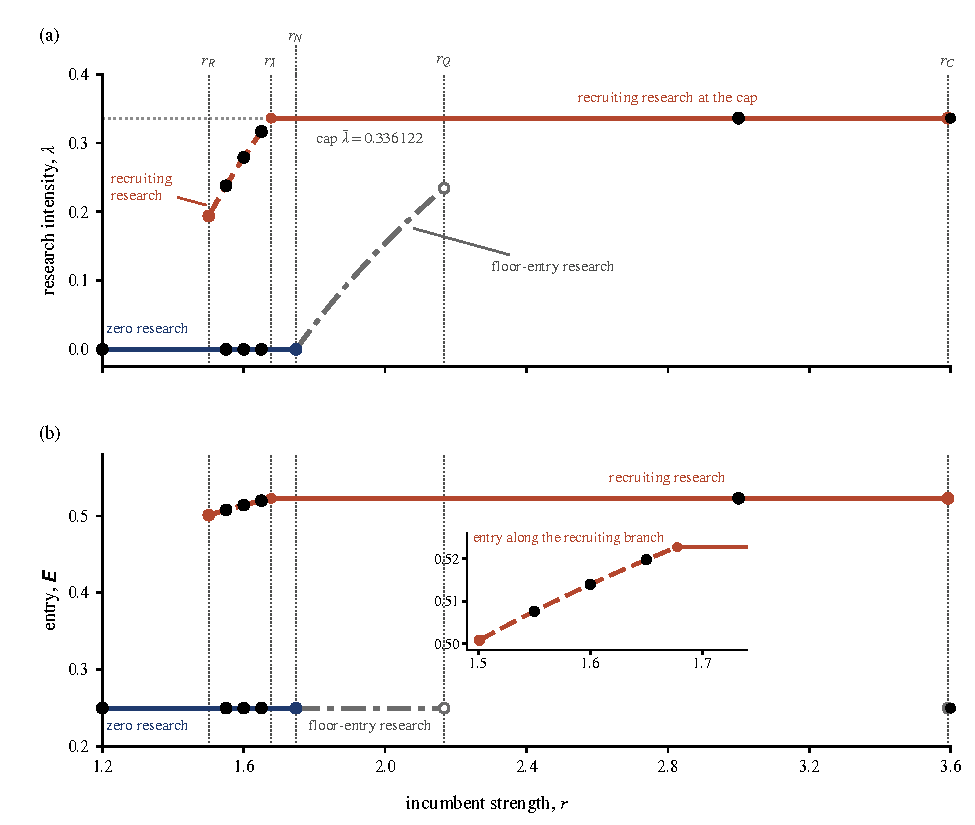
\includegraphics[width=0.62\linewidth]{../manuscript/figures/research.pdf}
\caption{Research and entry along the research branch \paper{Figure~3}. Gray band: \((r_N,r_U)\), where the equilibrium set
with research is not characterized.}\label{fig:09-research}
\end{figure}

\begin{panelnote}[Why the research branch starts later than \(r_A\)]
With a fixed presence, the informative branch starts at \(r_A=\reg{res_rA}\), where a purchase that recruits just covers
\(k\). With research, it must also cover the marginal research cost \(2a\lambda_E\), so the branch starts at
\(r_R=\reg{res_rR}\). The adjustment also differs: with a fixed presence the high class mixes; with research the
intensity adjusts and the high class buys with probability one after a success.
\end{panelnote}

\subsection{The admissible cap and cost, and the range of \texorpdfstring{\(\beta\)}{beta}}\label{sec:09_research-region}

\begin{resultbox}[The admissible cap and cost \paper{Prop.~A.2}]
Fix \(\beta=\reg{beta_B}\). Require the patterns of Proposition~4(b), with \(\lambda_E(r)<\lambda_R(r)<\lb\) at each intermediate strength.
These patterns have strict margins exactly when
\[\lambda_E(r_1)<\lb<\lambda_E(r_2),\qquad a_{\rm lo}(\lb)<a<a_{\rm up}.\]
The cost bounds are
\[
a_{\rm lo}(\lb)=\frac{\DT(1.65)\,m_{\lb}-k}{2\lb},\qquad a_{\rm up}=\frac{\DT(1.55)\,[1-\tau(1.55)]-k}{2\lambda_E(1.55)}.
\]
The cap strip is \((\reg{res_cap_lo},\reg{res_cap_hi})\). At \(\lb=\reg{res_cap}\) the cost window is
\((\reg{res_a_lo},\reg{res_a_up})\); at \(a=1/40\) the cap range is \((\reg{res_cap_lo_a},\reg{res_cap_hi})\).
\end{resultbox}

\begin{itemize}[leftmargin=2em]
\item \(\lb>\lambda_E(r_1)\): research at the cap recruits strictly at \(r_1\); otherwise every posterior there is at most
\(\tau(r_1)\). \(\lb<\lambda_E(r_2)\): research at the cap does not recruit at \(r_2\); otherwise C1 lifts entry above \(\rho\).
\item \(a<a_{\rm up}\) is \(\varphi_a(1.55)>0\): the purchase recruits strictly at 1.55, and, as \(a_{\rm up}<a_{\rm mono}\) makes
\(\varphi_a\) rise, at 1.60 and 1.65 too.
\item \(a>a_{\rm lo}(\lb)\) is \(F_{1.65}(\lb)>0\): research stays below the cap at 1.65, and so at 1.55 and 1.60, as
\(\lambda_R\) rises. \(a_{\rm lo}(\lb)=a\) exactly when \(\lb=\lambda_R(1.65)\); so the lower end of the cap range at
\(a=1/40\) is \(\lambda_R(1.65)=\reg{res_lambda_r165}\).
\item (U) at \(r_1\) and \(r_2\) adds nothing on the strip: both bounds \(a_U(r;\lb)=[\rho\DT(r)m_{\lb}-k]/\lb\) fall in
\(\lb\), and at \(\lb=\lambda_E(r_2)\) they are \reg{res_region_aU3_6} and \reg{res_region_a36_6}, both above
\(a_{\rm up}\). The window is nonempty on the whole strip, since \(a_{\rm lo}\) falls in \(\lb\) and
\(a_{\rm lo}(\lambda_E(r_1))=\reg{res_region_alo_0}<a_{\rm up}\).
\end{itemize}
The benchmark cap lies \reg{margin_res_caplo_B} and \reg{margin_res_caphi_B} inside the strip; the cost lies
\reg{margin_res_alo_B} and \reg{margin_res_aup_B} inside its window. The upper cap margin is the posterior margin
\(\tau(r_2)-M_{\lb}=\reg{margin_res_tau_r2_B}\) in another coordinate.

\paragraph{The range of \(\beta\).} Set the cap to the benchmark presence at each \(\beta\), \(\lb=\lambda_B(\beta)=u\beta/(1+u\beta)\)
with \(1+u=\eu\), and keep \(a=1/40\).
\begin{enumerate}[leftmargin=2em]
\item \(u_{\lb}=u\) for every \(\beta\), so \(M_{\lb}=\eu/(1+\eu)\) and \(m_{\lb}=1/(1+\eu)\) do not move, and the strip
condition holds for every \(\beta\).
\item (U) at \(r_1\) holds for every \(\beta\le1/3\), because \(\lambda_B\) rises in \(\beta\) and
\(\rho\DT(r_1)/(1+\eu)-k-a\lambda_B(1/3)=0.015719>0\). % verify/09_research.py
\item \(a_{\rm lo}=[\DT(1.65)/(1+\eu)-k]/[2\lambda_B(\beta)]\) falls in \(\beta\). So \(a_{\rm lo}<a\) exactly when
\(\lambda_B(\beta)>L=[\DT(1.65)/(1+\eu)-k]/(2a)=0.288653\), % verify/09_research.py
that is \(\beta>\beta_{\rm lo}=L/[u(1-L)]=\reg{res_beta_lo}\).
\item \(a_{\rm up}(\beta)\) falls in \(\beta\), because \(\partial\lambda_E/\partial\beta=(2\tau-1)(1-\tau)/\{\beta+(1-2\beta)(1-\tau)\}^2>0\),
and it exceeds \(a\) for \(\beta<\reg{res_beta_hi}\). \(a_{\rm mono}(\beta)\) falls in \(\beta\), with
\(a_{\rm mono}(1/3)=\reg{res_amono_third}>a\).
\end{enumerate}
So the patterns hold for every \(\beta\in(\reg{res_beta_lo},1/3]\), with entry \(\rho+(1-\rho)[\beta+(1/2-\beta)\lb]\) at
\(r_1\).

\subsection{Tie rules with research}\label{sec:09_research-ties}

\begin{resultbox}[Tie rules with research \paper{Remark~A.1}]
Research has a unique best response, and Proposition~4(b) needs no investor tie rule. Under the challenger rule CM, each intermediate
strength has one more equilibrium, the threshold equilibrium (T). Above \(r_U\) the tuple is unique under C1, and under CM
at every strength except the entry ceiling \(r_C=\reg{res_rC}\).
\end{resultbox}

In (T), research is \(\lambda_E(r)\), so the purchase posterior equals \(\tau\). The indifferent challenger prepares so that
entry after a purchase is \(e^*=(2a\lambda_E+k)/[\DT(1-\tau)]\). The purchase then earns \(e^*\DT(1-\tau)-k=2a\lambda_E\), so
\(V=a\lambda_E\) and (E7) holds. The preparation probability lies in \((0,1)\): \(e^*<1\) is \(\varphi_a>0\), and
\(e^*>\rho\) because \(\rho\DT(1-\tau)<\rho\DT/2<k<2a\lambda_E+k\). Entry is \(\rho+(e^*-\rho)[\beta+(1/2-\beta)\lambda_E]\):
\begin{center}\small
\begin{tabular}{@{}lccc@{}}
\toprule
 & \(r=\reg{str_r155}\) & \(r=\reg{str_r160}\) & \(r=\reg{str_r165}\)\\
\midrule
\(e^*\) & \reg{res_th_estar_r155} & \reg{res_th_estar_r160} & \reg{res_th_estar_r165}\\
Entry in (T) & \reg{res_th_entry_r155} & \reg{res_th_entry_r160} & \reg{res_th_entry_r165}\\
\bottomrule
\end{tabular}
\end{center}
Entry in (T) falls across the three strengths, while entry on the research branch rises. At \(r_C\), \(M_{\lb}=\tau(r_C)\):
CM admits every preparation probability after a purchase, each with its own competitive price, and entry fills
\([\rho,\reg{res_entry_cap}]\) while research stays at the cap.

\begin{caution}[Two threshold objects]
The threshold pair T of \Cref{sec:08_coexistence} has a fixed presence and a mixed purchase rate \(s^*\). The
threshold equilibrium (T) here has a pure purchase after a success and research \(\lambda_E\). Both put the purchase
posterior exactly at \(\tau\).
\end{caution}

Access to prices with research, and its effect on proceeds and surplus at \(r_1\), belongs to the welfare analysis
(\Cref{sec:11_welfare-access}).

The old guide had no research stage. Here presence responds to its expected return.
